\section{Methodological and Budget-Theory Details}
\label{app:theory_details}

This appendix retains the derivations, boundary examples, and implementation qualifications supporting Sections~\ref{sec:methodology} and~\ref{sec:budget}.

\subsection{Observe-then-commit structure and EFE scope}
\label{app:theory_setup}

\begin{figure}[tbp]
\centering
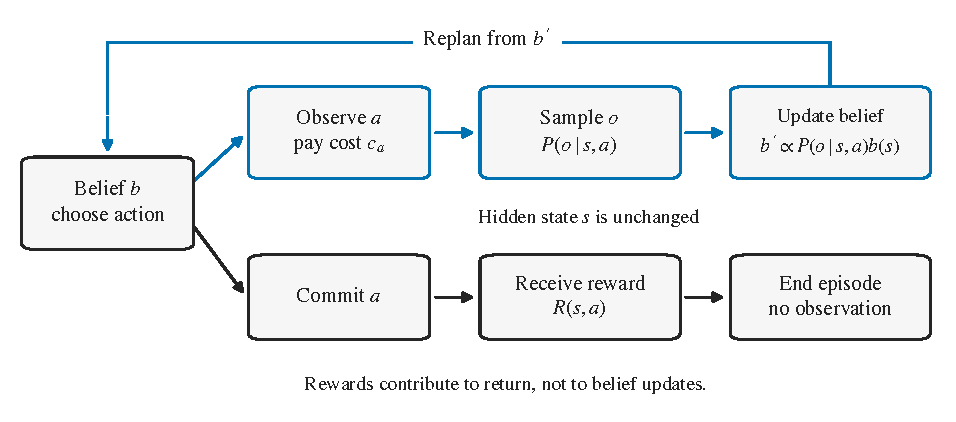
\includegraphics[width=\linewidth]{figures/fig_otc_loop.pdf}
\caption{The observe-then-commit decision loop, shown schematically. An observation incurs a cost and updates the belief about a hidden state that remains fixed. The agent then chooses again from the updated belief. A commit instead pays a state-dependent reward and ends the episode without emitting an observation. Rewards are not inputs to the belief update. The loop describes the episode, while the planner's finite horizon limits how far it looks ahead at each decision.}
\label{fig:otc_loop}
\Description{A current belief leads either to a paid observation, a posterior belief, and another decision, or to a terminal commit with state-dependent reward. The hidden state remains fixed along the observation loop. No arrow feeds reward into the belief update.}
\end{figure}

Proposition~\ref{prop:equivalence} covers one specific formulation of EFE, and we name what it does not cover before interpreting it. Equation~\ref{eq:efe_recursive} instantiates the recursive, closed-loop form of EFE associated with sophisticated inference \citep{friston2021,dacosta2020b}. In \citet{champion2024}'s taxonomy of EFE formulations this is the variant whose epistemic term is the expected information gain about the hidden state, evaluated recursively over belief trajectories. We establish the $w{=}1$ coefficient for that formulation only. Whether the same coefficient survives under the Free Energy of the Expected Future \citep{millidge2021}, generalised free energy \citep{parr2019}, the epistemic-prior variational treatment of \citet{devries2025}, or the Bethe-Lagrangian stationary point of \citet{kouw2026bethe} is not established here. A negative answer for any of them would narrow the scope of Proposition~\ref{prop:equivalence} without touching the budgeted results of Section~\ref{sec:budget}.

\paragraph{Reward-to-nats calibration.}
The equivalence needs an exchange rate between reward and information. The pragmatic term of EFE is an expected log-probability, measured in nats, while task reward arrives in whatever units the environment specifies, so identifying the two means fixing how many nats one reward unit is worth. Identifying pragmatic value with task reward chooses $P(o|C) \propto \exp(\beta R)$ with $\beta{=}1$ per reward unit, which sets that rate at one nat per reward unit. This identification is a convention adopted in assumption (i) of Proposition~\ref{prop:equivalence}, not a derivation, and the proposition is a statement about the recursion of Equation~\ref{eq:efe_recursive} as written, in which the pragmatic value of each scored outcome is its task reward and no normalizer appears. Deriving that recursion from a normalized preference distribution would add a term the recursion omits. Writing $Z = \sum_{o'} \exp(\beta R(o'))$ for the normalizer over the outcome space, $\ln P(o|C) = \beta R(o) - \ln Z$, and the constant $\ln Z$ is scored once per outcome, so a path that scores $T$ outcomes before it ends accumulates $-T \ln Z$. Observe-then-commit paths of different lengths score different numbers of outcomes, so that accumulated constant is policy-dependent and can change which of observing and committing minimizes the objective. Apart from the log-scoring case, in which the reward is itself a log probability so that $Z{=}1$ and the constant vanishes, it cancels only under a convention that scores the same number of outcomes on every path, for example a fixed-length construction in which an episode that has committed keeps emitting a null outcome of zero reward from an absorbing state at every remaining step, scored against one preference distribution over a common outcome space. We do not adopt such a construction, and the proposition's scope does not extend to a general normalized-preference derivation for variable-length episodes. Three things are therefore kept apart in this article. The exact case is Bernardo's, where the reward is itself a log probability and no normalizer arises. The proved case is the reward-based recursion, conditional on assumption (i). The empirical convention is one reward unit per bit, stated next. The choice has a consequence for scale. Rescaling all rewards by a positive factor $k$ (the factor written $\alpha$ in Proposition~\ref{prop:pi1}) at fixed $w$ induces the same policy as weight $w/k$ on the unscaled rewards, so $w{=}1$ is not scale-invariant, and the reward-maximizing weight $w^*_{\mathrm{ret}}$ (the subscript abbreviates return) scales as $w^*_{\mathrm{ret}}(k)\propto k$ (Appendix~\ref{app:reward_scaling}). Following \citet{bernardo1979}, the identification is exact when rewards are log scoring rules, that is, when the reward for an outcome is the log probability the agent assigned to that outcome, so that reward is already measured in nats and no unit conversion stands between the two terms. Our claim is weaker and operational. Within a fixed reward convention, the information-unit weight $w{=}1$ is a robust untuned default.

The implementation measures information in bits rather than nats (\texttt{scipy.stats.entropy} with $\mathrm{base}{=}2$), a constant-factor difference that we make explicit here. Every result reported as EFE ($w{=}1$) in this article runs the agent at $w{=}1$ in those bit units, that is, one reward unit per bit. Since one bit is $\ln 2$ nats, one reward unit per bit is one reward unit per $\ln 2$ nats, or $1/\ln 2$ reward units per nat, which is an effective nat-denominated weight of $1/\ln 2 \approx 1.44$. Running the same conversion in reverse, the exactly canonical nat-unit identification of Proposition~\ref{prop:equivalence} corresponds to $w = \ln 2 \approx 0.69$ in the implementation's bit units.

Whether that constant factor changes any reported result is settled directly in Appendix~\ref{app:nat_canonical}, which runs the exactly nat-canonical agent of Proposition~\ref{prop:equivalence}, $w{=}\ln 2$ in the implementation's bit units, under the Pareto sweep protocol of Section~\ref{sec:pareto} on all five swept environments (\texttt{results\_\allowbreak nat\_\allowbreak canonical\_\allowbreak check.csv}). On Tiger, Diagnosis, Bandit, and Testbed it is bit-identical to the implemented $w{=}1$ agent in reward, success rate, and observation count. Where that sweep's mean reward is exactly tied across adjacent swept weights, its reward-maximizing weight is reported as the closed range of tied grid weights, the reward-maximizing tied bracket. On Tiger and Diagnosis both weights lie inside it, and on Bandit, whose bracket has grid endpoints $[1, 2]$ and so contains $w{=}1$ but not $0.69$, the directly run nat-canonical agent attains the bracket's tied reward. Tileworld is the one swept environment where the base changes the policy, and there $w{=}1$ remains Pareto-dominated by $w{=}20$ under either convention.

\subsection{Two-state thresholds and their empirical scope}
\label{app:theory_thresholds}

The two parts of Proposition~\ref{prop:nearopt} concern distinct horizons. We retain the derivation and descriptive comparisons here.

\begin{proof}[Proof sketch]
\emph{Part (a).} At $H{=}1$, the agent observes once and commits. A Planning+IG agent with weight $w$ observes iff $-c + w \cdot I(b) + \mathbb{E}_o[\max_i \mathbb{E}_{b'_o}[R_i]] > \max_i \mathbb{E}_b[R_i]$, where the left side is the observe-then-commit value and the right side is the immediate commit value. For the uniform prior, the immediate commit value is $(R^+ + R^-)/2$. After one observation, the posterior concentrates. With probability $p$ the agent is correct, yielding expected commit value $p \cdot R^+ + (1-p) \cdot R^-$. The net gain from observing is $(p - \frac{1}{2})(R^+ - R^-) - c + w \cdot I_{\max}$. Setting this to zero gives $w^*_{\mathrm{thresh}} = [c - (p-\frac{1}{2})(R^+ - R^-)]/I_{\max}$. Substituting $R^- = -\alpha R^+$ yields the second form. When $\alpha \gg 1$, the marginal reward improvement $(p - \frac{1}{2})(1 + \alpha)R^+$ dominates the cost $c$, making $w^*_{\mathrm{thresh}}$ negative, so the agent should observe at any $w \geq 0$, including $w{=}1$.

\emph{Part (b).} Fix the post-first-observation belief $b{=}(p,1{-}p)$. The agent prefers a second observation over committing when $-c + w \cdot I(b) + \mathbb{E}_{o'}[\max_i \mathbb{E}_{b'_{o'}}[R_i]] > \max_i \mathbb{E}_b[R_i]$, i.e., when $w > (c - \mathrm{VoI}_2(b))/I(b)$ whenever $\mathrm{VoI}_2(b) < c$. That cutoff is $w^*_{\mathrm{over}}$. Combining both inequalities yields the $H{=}2$ near-optimality interval.
\end{proof}

Under the paper's reward convention, $w{=}1$ lies in this interval for Tiger, the one tabulated instance that is genuinely two-state with $|R^-| > R^+$ and so falls under the proposition as stated. For Diagnosis and Tileworld, which are multi-state, multi-action environments outside the proposition's stated hypothesis, the same thresholds are applied heuristically to a two-state reduction, for which no formal correspondence is proved. The reduction takes each environment's observation accuracy as $p$, its per-observation cost as $c$ (a test on Diagnosis, a scan on Tileworld), and its correct and incorrect commit rewards as $R^+$ and $R^-$, and it keeps nothing of the state and observation-action counts. Diagnosis and Tileworld share all four of those values (Appendix~\ref{app:envs}), which is why their two rows in the table coincide. Table~\ref{tab:alpha_eta} provides a descriptive comparison against Proposition~\ref{prop:nearopt} on this basis. It reports $\alpha$, $\eta$, the lower and upper thresholds $w^*_{\mathrm{lo}}$ and $w^*_{\mathrm{hi}}$, and the observed reward-maximizing weight from the Pareto sweep (Section~\ref{sec:pareto}). The table writes Part (a)'s $w^*_{\mathrm{thresh}}$ as $w^*_{\mathrm{lo}}$ and Part (b)'s $w^*_{\mathrm{over}}$ as $w^*_{\mathrm{hi}}$.

\begin{table}[ht]
\centering
\caption{Reward asymmetry ($\alpha$), informativeness ($\eta$ in nats), lower observation threshold $w^*_{\mathrm{lo}}$, upper over-observation threshold $w^*_{\mathrm{hi}}$, and the observed reward-maximizing weight (or bracket) $w^*_{\mathrm{ret}}$ from a fresh Pareto sweep (Section~\ref{sec:pareto}, the eleven-point grid $w \in \{0.01, 0.1, 0.5, 1, 2, 5, 10, 20, 50, 100, 200\}$, 5 seeds $\times$ 500 episodes, \texttt{results\_\allowbreak pareto\_\allowbreak sweep.csv}). Where the sweep's reward is exactly tied across several adjacent grid weights, $w^*_{\mathrm{ret}}$ is reported as the closed range of tied grid weights rather than an arbitrary point within it. That range is a flat set of maximizers, the analogue of the level set of Definition~\ref{def:pi3}, not a crossing bracket. Only Tileworld has a genuinely unique argmax in this grid. Thresholds in nats. The $w{=}1$ column asks about the canonical nat-denominated weight, while the implemented bit-denominated agent corresponds to $1.44$ nats (see text). Bandit omitted as multi-arm, so Prop.~\ref{prop:nearopt} does not apply directly.}
\label{tab:alpha_eta}
%% Numbers in this table are produced by experiments/run_thresholds.py (analytic columns) + experiments/run_pareto.py (w*_ret brackets)
\begin{tablebody}
\begin{tabular}{lcccccc}
\toprule
Environment & $\alpha$ & $\eta$ & $w^*_{\mathrm{lo}}$ & $w^*_{\mathrm{hi}}$ & $w{=}1$ in $(w^*_{\mathrm{lo}},w^*_{\mathrm{hi}})$? & $w^*_{\mathrm{ret}}$ \\
\midrule
Testbed & $1.0$ & $1.31$ & $-3.06$ & $1.01$ & Nat units only (see text) & $[0.01, 0.5]$ (tied) \\
Tiger & $10.0$ & $0.27$ & $-138.66$ & $6.89$ & Yes & $[0.01, 20]$ (tied) \\
Diagnosis & $5.0$ & $0.19$ & $-88.20$ & $7.91$ & Yes & $[0.5, 20]$ (tied) \\
Tileworld & $5.0$ & $0.19$ & $-88.20$ & $7.91$ & Yes & $20$ (unique) \\
\bottomrule
\end{tabular}
\end{tablebody}
\end{table}

Table~\ref{tab:alpha_eta} shows two patterns. On the three high-asymmetry environments (Tiger, Diagnosis, Tileworld) $w{=}1$ sits comfortably inside the interval in either unit convention, whereas Testbed sits on the interval's upper edge and on the boundary of the proposition's hypothesis, and we take Testbed first. On Testbed, the lower threshold is negative and the upper bound is tight ($w^*_{\mathrm{hi}} \approx 1.01$). Nat-denominated $w{=}1$ sits just inside, while the implemented agent's bit-denominated $w{=}1$ corresponds to $1.44$ nats and falls outside the interval. This is consistent with the over-exploration observed relative to the reward-maximizing bracket $w^*_{\mathrm{ret}} \in [0.01, 0.5]$ (Appendix~\ref{app:testbed}). Under the sweep protocol at $H{=}4$, however, the nat-canonical agent of Appendix~\ref{app:nat_canonical} over-explores exactly as the bit-denominated agent does, matching it in reward, success rate, and observation count (\texttt{results\_\allowbreak nat\_\allowbreak canonical\_\allowbreak check.csv}), so the interval's tight upper endpoint separates the two conventions on paper but not in measured behavior at that horizon. Testbed's $\alpha{=}1.0$ sits at the boundary of Proposition~\ref{prop:nearopt}'s strict assumption $|R^-| > R^+$. Its row is included descriptively rather than as an instance of the proposition.

The second pattern is the high-asymmetry one. Tiger, Diagnosis, and Tileworld have $w^*_{\mathrm{lo}} \ll 0$ and $w^*_{\mathrm{hi}} \approx 7$--$8$. The near-optimality interval between those thresholds is derived at $H{=}2$, and the multi-step case beyond $H{=}2$ is harder to analyze because thresholds shift with belief. Read as a prediction about the sweep, the interval says that $w{=}1$ lands among the reward-maximizing weights wherever it lies inside the interval. On Tiger and Diagnosis the prediction is borne out, since $w{=}1$ sits inside the reward-maximizing tied bracket. On Tileworld it is not. Tileworld's reward-maximizing weight is uniquely $w{=}20$ in the implementation's bit units ($28.9$ nats), which lies above the interval's nat-denominated upper endpoint of $7.91$, and $w{=}1$ is Pareto-dominated there.

\paragraph{Extension to discounting.} Discounting preserves the $\rho$-POMDP equivalence with $\rho(b,a) = I_a(b)$, but it changes the balance between the two terms along a branch. The measured net effect runs toward fewer observations rather than more. With $\gamma < 1$, the recursive EFE becomes $\mathcal{G}(\text{obs}_k) = c_k - I_k(b) + \gamma\, \mathbb{E}_o[\min_a \mathcal{G}(a, b'_o)]$, giving $V(\text{obs}_k) = -c_k + I_k(b) + \gamma\, \mathbb{E}_o[\max_a V(a, b'_o)]$. The information gain term $I_k(b)$ appears undiscounted at the current step, while future values are discounted. The intuition is that the information gain at a node is credited immediately, while the reward that information eventually buys arrives only at the commit action and is discounted by $\gamma$ raised to the number of steps remaining until then. In the undiscounted case ($\gamma{=}1$), the immediate information gain and the commit reward it later buys are weighted equally at every depth. With $\gamma < 1$ the epistemic share of an observe branch's value therefore rises with the length of the branch. This does not make the agent more exploratory overall, because discounting also shrinks the whole observe branch relative to committing now, and the measured effect runs the other way, with EFE's observation count on Diagnosis falling from $9.68$ at $\gamma{=}1$ to $5.83$ at $\gamma{=}0.95$ (Table~\ref{tab:discount}). Appendix~\ref{app:discount} compares EFE with Planning, the reward-only planner of the same horizon, across discount factors, and Section~\ref{sec:discussion} takes up the consequence. On environments with several observation actions EFE's advantage requires $\gamma \geq 0.99$, because heavier discounting truncates the effective horizon.

\subsection{State-preservation proof and destructive sensing}
\label{app:theory_factored}

\begin{proof}[Proof sketch]
When action $a$ preserves $s_{\mathrm{hid}}$, the transition on the hidden component is $T_{\mathrm{hid}}(s'_{\mathrm{hid}} | s_{\mathrm{hid}}, a) = \delta(s'_{\mathrm{hid}} = s_{\mathrm{hid}})$. The belief update over $s_{\mathrm{hid}}$ is then $b'(s_{\mathrm{hid}}) \propto O(o \mid s_{\mathrm{hid}}, a)\, b(s_{\mathrm{hid}})$, depending only on the observation likelihood, identical to the observe-then-commit case. The posterior that would incorporate transitions, $b'_{o,T}$, coincides with the observation-only posterior $b'_o$, so $D_{\mathrm{KL}}[b'_{o,T} \| b'_o] = 0$. For observation actions, EFE reduces to cost minus information gain plus expected continuation, matching the $\rho$-POMDP Bellman equation with $\rho = I_a(b)$. For navigation actions, the observation is uninformative ($I_a(b) = 0$), giving $\rho = 0$.
\end{proof}

Proposition~\ref{prop:factored} extends the formal bridge from observe-then-commit to any POMDP where the hidden state is preserved by information-gathering and navigation actions. Where the observe-then-commit argument had a single run of observations followed by one commit, the agent here may interleave observation, navigation, and exploitation in any order. The planner enumerates action sequences as a tree over belief states, using the recursive tree search of Equation~\ref{eq:efe_recursive} extended with navigation and exploitation branches. At each decision point, the EFE-as-$\rho$ equivalence holds on every branch of that tree made up of observation and navigation actions. Because navigation actions never touch the hidden state, interleaving them with observation actions does not disturb the equivalence, and $\rho_{\mathrm{EFE}}$ is well defined along any sequence of actions drawn from $\mathcal{A}_{\mathrm{obs}} \cup \mathcal{A}_{\mathrm{nav}}$, regardless of how many such actions precede a given decision.

Exploitation actions are not covered by Proposition~\ref{prop:factored}, and they carry no belief-dependent utility term for two separate reasons, depending on whether they end the episode. An exploitation action that ends the episode, such as exit, carries $\rho_{\mathrm{EFE}} = 0$ for the reason Proposition~\ref{prop:equivalence} gives for commit actions, that termination leaves no successor belief to score. An exploitation action that does not end the episode, such as sampling a rock, yields a reward that depends on the hidden state. That its reward already enters the objective is not by itself a reason for it to carry no epistemic term, because a payoff that depends on $s_{\mathrm{hid}}$ can reveal $s_{\mathrm{hid}}$. The reason is instead an assumption of the formal model that the benchmark shares. Rewards are not observations. The belief is conditioned on the observation symbol alone, a non-terminal exploitation action emits an uninformative observation, and its payoff is never fed back into the belief, so its expected information gain under the model's observation channel is zero and $\rho_{\mathrm{EFE}} = 0$ follows from the definition of $I_a(b)$ rather than from a separate stipulation. In RockSample the implemented agents mark a sampled rock as sampled, which removes its quality from every later decision because re-sampling earns nothing, and they do not infer the quality from the sampling payoff (\texttt{rho\_\allowbreak aif/\allowbreak agents/\allowbreak rocksample\_\allowbreak agents.py}). A model in which the payoff of an exploitation action is itself observed and conditioned on would give that action a positive information gain, and the equivalence would then have to include an epistemic term for it. We do not treat that case. Whatever a non-terminal exploitation action does to the visible state is handled at the next decision point, where replanning starts from the resulting belief and recomputes $\rho_{\mathrm{EFE}}$ fresh. The coupling term $\Delta_T$ only reenters if an action nominally classified as observation or navigation in fact changes $s_{\mathrm{hid}}$, which Definition~\ref{def:factored} rules out by construction rather than by approximation.

The extension therefore covers RockSample's check and navigation actions. Beyond that benchmark, it covers mobile sensor placement and sequential testing with spatial access costs, domains where the agent must navigate to observation locations before gathering information. Section~\ref{sec:rocksample} exercises this extension empirically across four RockSample instances, and empirical agreement exercises the algebraic result but does not prove it.

The factored observation structure is common in practice whenever the quantity being measured is static or slow-changing relative to the decision horizon (Table~\ref{tab:taxonomy}). The key requirement, that $T_{\mathrm{hid}}(s'_{\mathrm{hid}} | s_{\mathrm{hid}}, a) = \delta(s'_{\mathrm{hid}} = s_{\mathrm{hid}})$ for observation and navigation actions, breaks when information-gathering itself alters the hidden state. In such settings the coupling term may be nonzero, $\Delta_T \neq 0$ at some beliefs, and the identity $\rho_{\mathrm{EFE}}(b,a) = I_a(b)$ behind the information-unit-weight equivalence (the EFE-as-$\rho$ equivalence at $w{=}1$) then fails in general. We discuss this further in the limitations paragraph of Section~\ref{sec:discussion}. Example~\ref{ex:destructive} makes precise what fails and how badly.

\begin{remark}[The scope restriction is on the reduction, not on what EFE can price]
\label{rem:transition-aware}
Example~\ref{ex:destructive} shows a failure of the factored $\rho$-POMDP reduction, not a failure of Expected Free Energy. For any action $a$ that violates Definition~\ref{def:factored}'s state-preserving hypothesis ($\Delta_T(b,a) \neq 0$), replacing the naive epistemic term $I_a(b) = \mathbb{E}_{o \mid a} D_{\mathrm{KL}}[Q(s_{\mathrm{hid}} \mid o, a) \,\|\, Q(s_{\mathrm{hid}} \mid a)]$, computed from the pre-transition posterior $b'_o$, with the transition-aware term computed from the correct joint posterior $b'_{o,T}(s') \propto \sum_{s} T(s' \mid s, a)\, O(o \mid s, a)\, b(s)$, under this article's observe-then-transition timing convention where the observation is emitted from the pre-transition hidden state and the dynamics then act, removes the illusory information credit. In Example~\ref{ex:destructive} the post-transition state is degenerate, the transition-aware epistemic term vanishes, and the substitution recovers the reward-only Bellman value $V_{\mathrm{true}}(a_D)$ exactly. In general it restores the correct belief dynamics while still crediting whatever genuine post-transition information the action carries, so it prices destructive sensing correctly rather than reducing to reward-only planning. Propositions~\ref{prop:equivalence}--\ref{prop:factored} therefore delimit which $\rho$-POMDPs the factored reduction targets (those with $\Delta_T \equiv 0$ on information-gathering actions), not which decision problems Expected Free Energy can correctly evaluate. EFE's epistemic term is defined over post-transition beliefs by construction, so it prices destructive sensing correctly once the epistemic term is recomputed from transition-aware predictive and posterior distributions as above. The coupling term $\Delta_T$ itself is a diagnostic of when the factored hypothesis fails, and we have not shown it to be an additive correction to the EFE value or a bound on decision error. We leave a transition-aware treatment of the budgeted machinery of Section~\ref{sec:budget}, and any perturbation bound in terms of $\Delta_T$, as future work (Section~\ref{sec:discussion}).
\end{remark}

\begin{table}[ht]
\centering
\caption{Taxonomy of real-world POMDPs by factored observation structure. Factored settings preserve the hidden state under observation and navigation actions, while non-factored settings do not.}
\label{tab:taxonomy}
\begin{tablebody}
\begin{tabular}{p{3.6cm}p{4.2cm}}
\toprule
\textbf{Factored} ($\Delta_T{=}0$) & \textbf{Non-factored} ($\Delta_T{\neq}0$) \\
\midrule
Non-destructive testing & Destructive testing (drilling) \\
Medical imaging (CT, MRI) & Biopsy / tissue sampling \\
Structural inspection & Active interventions \\
Environmental monitoring & Predator--prey (target moves) \\
Security screening & Chemical testing (consumes sample) \\
Mineral exploration & Quantum measurement \\
Mobile sensor networks & Adversarial surveillance \\
\bottomrule
\end{tabular}
\end{tablebody}
\end{table}

\subsection{Agent specifications and weight selection}
\label{app:theory_agents}

Planning+IG is the critical baseline. It uses the same tree search as the EFE agent with an additive information-gain (IG) bonus at the same horizon, meaning that at every node of the tree the value of an observation action is its reward-only value plus $w$ times the expected information gain $I_a(b)$ of that observation. Planning+IG is also this article's instance of a construction that two lines of prior work share, namely POMDPs with information rewards (POMDP-IR) and $\rho$-POMDPs with an information-gain reward \citep{spaan2015,araya2010}. \citet{satsangi2018} show that these two formulations are equivalent, so Planning+IG stands in for both. A reader from the active-perception literature should therefore read Planning+IG at a tuned weight as the familiar baseline from that tradition rather than as a construction specific to this article. By Proposition~\ref{prop:equivalence}, the EFE agent is exactly Planning+IG with $w{=}1$, so any difference between EFE and Planning+IG at a tuned weight, in either direction, is attributable to the weight choice rather than a different mechanism. That weight-only reading presumes the EFE implementation computes the epistemic term it claims to, so the EFE computation itself is checked for consistency against \texttt{pymdp} \citep{heins2022}, a reference Python library for active inference (Appendix~\ref{app:pymdp}). This is a qualitative agreement check on the epistemic term, not a certified numerical equivalence.

The Epistemic-only agent is the ablation that removes the pragmatic term. It sets $\mathcal{G}(\text{commit}) = 0$, removing reward awareness from the decision of when to commit, so that the comparison between observing and committing sees only observation costs and information gain. Once that comparison favors committing, the agent takes the commit action for the state its belief rates most probable, the belief-argmax commit, which is how it can still succeed once its belief is sharp. Success, for an observe-then-commit environment, is the fraction of episodes in which the agent's commit is correct. On Tiger, Diagnosis, Bandit, and Tileworld no observation's information gain alone clears its cost, so the agent commits immediately from its prior and succeeds at the chance rate, the accuracy the prior alone affords (Section~\ref{sec:results}, per-agent numbers in Appendix~\ref{app:full_tables}). Testbed is the exception, since its observation is cheap enough that information gain alone clears the cost, and there the ablation matches reward-only Planning exactly (Appendix~\ref{app:testbed}). The pragmatic term is what makes commit timing reward-aware, and the four chance-level environments show what its removal costs.

Four of the remaining baselines need a brief description here. Myopic ($\rho{=}0$, $H{=}1$) has no epistemic term at all, yet it observes on many environments. It does so because its one-step lookahead compares committing now against observing once and then committing, so it can see when a commit made after an observation is worth more than one made now. That difference is the instrumental value of information (VoI) of the observation, and Myopic observes for that reason rather than because of an epistemic bonus. The Greedy baseline provides a no-information lower bound in RockSample and Structural Inspection, both specified in Section~\ref{sec:experiments}. In RockSample it moves to rocks and samples them without first checking whether they are good. In Structural Inspection it declares a diagnosis for each component without running any test, so its declarations rest on the prior alone. We also include an observe-then-commit baseline built on information-directed sampling (IDS) \citep{russo2014}, which picks the observation action that minimizes its information ratio, the squared expected regret of taking that action divided by the information the action yields about the optimal commit (results in Appendix~\ref{app:ids}). The fourth baseline warrants a naming note. The posterior-vote baseline draws $100$ states from the belief, finds for each sampled state the action that would be optimal if that state were the true state, and takes the majority vote over those actions. As the sample count grows, this vote approaches the most-likely-state rule, which acts as if the belief's most probable state were the true state. It is not Thompson sampling, and we do not claim it as such. Thompson sampling draws a single state and acts optimally for that one draw, so the frequency with which it takes each action matches the belief's probability that the action is optimal, whereas the hundred-sample majority vote collapses toward a single action. The committed CSVs record it under the legacy label \texttt{ThompsonSamplingAgent}, retained so the artifacts stay stable.

Two of the six core agents carry a weight $w$ that must be set. They are Info Gain and Planning+IG (Table~\ref{tab:agents}). We report two tuning criteria for that weight, a success-maximizing criterion used in the main tables and a reward-maximizing criterion used in the Pareto analysis. In the main tables, the tuned weight for Info Gain and Planning+IG is the success-maximizing weight chosen by grid search over $\{0.1, 0.5, 1, 2, 5, 10, 20, 50, 100\}$. It is written $w^*_{\mathrm{succ}}$ in the results tables and $w^*$ where the criterion is clear from context. Each grid point is evaluated on 200 episodes, except on Tileworld, where 100 episodes are used because its computational cost per episode is an order of magnitude higher than that of the other observe-then-commit environments. Every grid point is evaluated on one common tuning stream, seed $7$, disjoint from the five evaluation seeds and reset for each candidate so that candidates face the same episodes, and ties go to the smallest weight reaching the maximum (\texttt{tune\_\allowbreak info\_\allowbreak gain\_\allowbreak weight} in \texttt{experiments/\allowbreak run\_\allowbreak experiment.py}). Each tuned weight is therefore a selection on one stream of $200$ or $100$ episodes and carries that stream's sampling noise. Seed $7$ is also the first held-out seed of Section~\ref{sec:budget_frontier}, which evaluates only the calibrated family and never a tuned baseline. This tuned baseline weight is a different quantity from the shadow price $w^*(B)$ of Section~\ref{sec:budget} and from the thresholds of Proposition~\ref{prop:nearopt}, which share the star notation. The Pareto analysis (Section~\ref{sec:pareto}), which traces mean reward against success as $w$ varies, sweeps a wider eleven-weight grid, listed in that section, and reports the reward-maximizing weight $w^*_{\mathrm{ret}}$. The two criteria can select different weights, and both are reported so that a reader can see which one a comparison uses. Section~\ref{sec:budget} then offers a third way to fix the weight, reading it off a sensing budget as the bracket of adjacent grid weights between which the agent's induced sensing usage crosses that budget.

\subsection{Proof and numerical check of the usage-onset corollary}
\label{app:theory_budget_proofs}

The scale-equivariance and comparative-statics proofs appear with Propositions~\ref{prop:pi1} and~\ref{prop:pi2}. We give the onset argument and its implementation check here.

\begin{proof}
At $H{=}1$ the only two plans are commit now and observe once then commit, and Proposition~\ref{prop:nearopt} establishes the observe plan is preferred iff $w > w_{\mathrm{thresh}}$. Consequently $U(w) = \mathbb{1}[w > w_{\mathrm{thresh}}]$ exactly for this single observe-or-commit decision, so $U$ is $0$ below $w_{\mathrm{thresh}}$ and $1$ above it. For any $B \in (0,1)$ the supremum of the weights with $U(w) < B$ that precede a weight with $U(w) \ge B$ is therefore $w_{\mathrm{thresh}}$, which is the stated crossing threshold, and a grid whose sampled usages straddle $B$ returns a bracket whose closed enclosure contains $w_{\mathrm{thresh}}$. The claim is about this $H{=}1$ decision, not about the receding-horizon usage curves of Section~\ref{sec:budget_experiments}, which take many values and need not be monotone.
\end{proof}

The corollary is verified numerically (\texttt{TestProp2OnsetExact} in \url{tests/test_budget.py}). The check runs the implemented $H{=}1$ planner over whole episodes rather than over the single decision the corollary analyzes. Within an episode that planner re-plans after each observation and is free to observe again before committing, so the test asserts the location of the onset rather than a usage of exactly $1$. Usage is exactly $0$ at $0.9\,w_{\mathrm{thresh}}$ and at least $1$ at $1.2\,w_{\mathrm{thresh}}$ on a positive-threshold Testbed with observation accuracy $p{=}0.6$, observation cost $c{=}0.3$, and correct and incorrect commit rewards $R{=}\pm 1$, whose threshold is $w_{\mathrm{thresh}} \approx 3.44$ in the implementation's bit units. Those bit units are the convention of the swept weight grid, and the calibration paragraph following Proposition~\ref{prop:equivalence} gives the conversion to the nat units of the proposition. Section~\ref{sec:prop2exp} extends the check to a refined weight grid on two such environments.

\subsection{Proof and implementation scope of the online controller}
\label{app:theory_controller}

\begin{figure}[tbp]
\centering
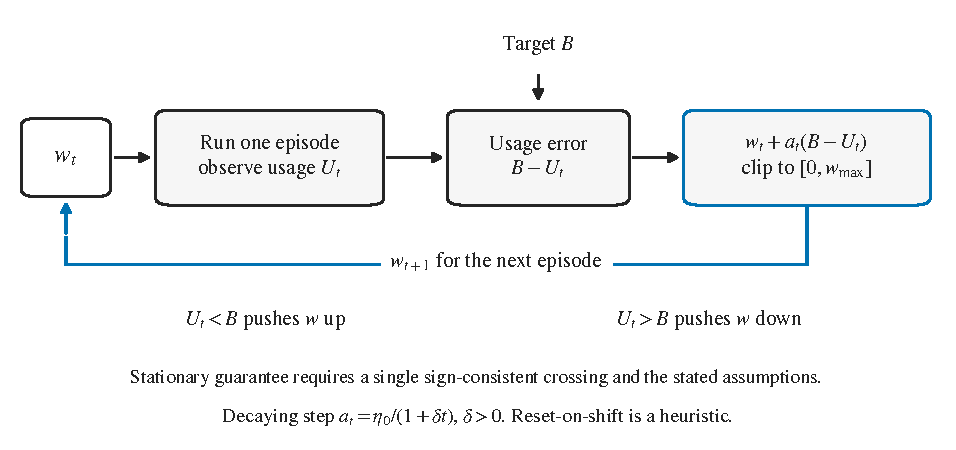
\includegraphics[width=\linewidth]{figures/fig_dual_feedback.pdf}
\caption{One episode of the projected weight controller, shown schematically. The current weight produces an observed usage $U_t$. The controller adds a step proportional to $B-U_t$ and clips the result to $[0,w_{\max}]$. Underspending raises the weight and overspending lowers it, subject to clipping. This direction corrects usage under the sign-consistent crossing assumptions of Proposition~\ref{prop:pi5}. The proposition covers the projected decaying-step update in a stationary setting under its four stated conditions, not arbitrary usage curves or the reset-on-shift heuristic.}
\label{fig:dual_feedback}
\Description{A loop runs from the current information weight through one episode and its observed usage to a signed budget error, then a projected update and the next episode's weight. Labels show that underspending raises the weight and overspending lowers it. Projection bounds the weight between zero and its declared maximum.}
\end{figure}

Three versions of this controller appear in the article, and it matters which one each statement is about. The first is the projected decaying-step controller, the recursion~\eqref{eq:dual_update} with a finite $w_{\max}$ and $\delta > 0$. It is the algorithm Proposition~\ref{prop:pi5} covers, and it is the algorithm every reported run executes, with $w_{\max}{=}100$, the top of the swept weight grid, and $\delta{=}0.02$ (\texttt{DualWeightAgent} in \texttt{rho\_\allowbreak aif/\allowbreak agents/\allowbreak dual\_\allowbreak descent.py} with \texttt{max\_\allowbreak weight} set, wrapping \texttt{dual\_\allowbreak update} in \texttt{rho\_\allowbreak aif/\allowbreak budget.py}). No reported iterate exceeded $3.1$, more than an order of magnitude below $w_{\max}$, so the upper projection never bound, but it is in force. The second is the released library default, which sets no upper projection and uses a constant step ($\delta{=}0$). The proposition covers neither of those two departures, and no result in this article is reported for that default. The third is the reset-on-shift heuristic described below, which the proposition also does not cover.

The recursion originates with \citet{robbins1951}, with classical almost-sure extensions due to \citet{blum1954}. \citet{kushner1978} treats constrained stochastic approximation. We prove the stated bounded scalar case directly, including discontinuous usage curves. Let $\mathcal{F}_t$ be the history before episode $t$, $e_t=w_t-w^*$, and $M(w)=U(w)-B$. By (ii), $\mathbb{E}[U_t\mid\mathcal{F}_t]=U(w_t)$ and $(B-U_t)^2$ is bounded by a constant $C$. Projection onto an interval containing $w^*$ cannot increase distance from $w^*$, so
\[
\mathbb{E}[e_{t+1}^2\mid\mathcal{F}_t]
\le e_t^2-2a_t e_t M(w_t)+C a_t^2.
\]
Condition (iii) gives $e_t M(w_t)\ge0$, also when $w_t=w^*$ without requiring $M(w^*)=0$. Thus $Y_t=e_t^2+C\sum_{k\ge t}a_k^2$ is a nonnegative supermartingale and converges almost surely. Summing the expected drift inequality gives $2\,\mathbb{E}[\sum_t a_t e_t M(w_t)]\le\mathbb{E}[Y_0]<\infty$, so that nonnegative series is finite almost surely. Since the tail $\sum_{k\ge t}a_k^2$ vanishes, $e_t^2$ has an almost-sure limit. If it were positive, the bounded interval and condition (iv) would keep $e_t M(w_t)$ bounded away from zero eventually, contradicting $\sum_t a_t=\infty$. Hence $w_t\to w^*$ almost surely.

The running-average claim follows from that convergence. Because $w^*$ is interior and the increments $a_t (B - U_t)$ vanish, usage being bounded by (ii), the projection is inactive from some episode on, so $\sum_t a_t (B - U_t)$ converges, its partial sums being differences of the convergent iterates. Since $1/a_t = (1 + \delta t)/\eta_0$ increases to infinity, Kronecker's lemma gives $a_n \sum_{t<n} (B - U_t) \to 0$, and because $n\,a_n \to \eta_0/\delta > 0$ under that schedule, the one property of it the running-average claim uses, this is $\frac{1}{n}\sum_{t<n} (B - U_t) \to 0$ almost surely. Under a constant step, which no reported run uses, the recursion need not converge to a point. The standard constant-step stochastic-approximation intuition is that the iterate is instead held near $w^*$ in a neighborhood whose width shrinks with the step size, and that this residual motion is the mechanism that lets the controller re-adapt after the budget or environment shifts. Making it precise requires constant-step tracking arguments (stationary-distribution or moment bounds under drift and noise assumptions) that we do not develop here. Section~\ref{sec:dual_multiseed} assesses re-adaptation under reward-scale shift empirically on the decaying schedule, to which the same intuition applies through whatever step size is left at the moment of the shift. That section also runs the reset-on-shift variant, described next.

The \emph{reset-on-shift} variant of the controller watches the usage of the most recent episodes. When that usage persistently misses the budget after the step size has already decayed below half its initial value, it restarts the episode counter $t$ in the step schedule of~\eqref{eq:dual_update} at zero, so that the step size jumps back to $\eta_0$ and the controller can move quickly again. Resetting the decay clock mid-run in this way breaks the trajectory into a sequence of Robbins--Monro-style segments stitched together by a change-detection heuristic, rather than a single non-increasing step schedule. The proposition therefore does not cover the reset-on-shift variant when that variant is treated as a single run.

The proposition's scope has one further limit. It is conditional on a single, sign-consistent crossing of $B$. It is silent when $U$ crosses $B$ more than once, which the discussion after Proposition~\ref{prop:pi2} shows to be a real possibility, since the usage staircase need not be monotone.

\subsection{Relationship to constrained planning and experimental design}
\label{app:theory_positioning}

Our weight $w$ is calibrated within the Planning+IG family so that expected sensing usage meets a stated target, and it is not the Lagrange multiplier of the usage cap in problem~\eqref{eq:budgeted} (Section~\ref{sec:budget_theory}). We do not claim novelty for the underlying idea of adjusting a scalar price until a resource quantity meets a target. That idea is classical in constrained MDPs \citep{altman1999}, rational inattention \citep{sims2003,matejka2015}, and SAC temperature auto-tuning \citep{haarnoja2018sac}. Sims \citep{sims2003} models agents with finite Shannon capacity, and Mat\v{e}jka and McKay \citep{matejka2015} derive discrete-choice logits from costly information acquisition. Both take an information-processing constraint as the primitive. We take an operational sensing budget as the primitive and recover the Planning+IG weight that implements it. \citet{kim2011cpomdp} extend constrained dynamic programming to partial observability directly, showing that optimal constrained POMDP policies can require randomization and giving point-based dynamic programming over belief and admissible-cost pairs. Their method is not a Lagrangian one. Point-based solvers represent the value function by a set of vectors over beliefs and discard the dominated ones at each backup, and their method enforces the cost bound inside that pruning step rather than pricing it. The dominated vectors are pruned exactly with a minimax quadratically constrained program and approximately with a linear program at each collected belief point. Their constraints are exogenous costs enforced offline. The usage target here is also stated on a non-epistemic quantity, the count of sensing actions or their cumulative cost, rather than on information gained. What differs is that the price $w$ on belief-computed information gain is set offline by the grid solve of Section~\ref{sec:budget_solve} or adjusted online by the controller of Section~\ref{sec:pi5} until expected sensing usage meets the target.

The single-price receding-horizon family is the set of policies that run one scalar weight $w$ throughout an episode. It includes the per-episode mixture of Definition~\ref{def:pi3}, which randomizes between the two bracket endpoints from one episode to the next. This family attains the usage budget in expectation. We do not claim it is reward-optimal among all budget-feasible policies. An exact solver in the style of \citet{kim2011cpomdp} can randomize belief-dependently and may attain strictly higher constrained reward, particularly at gap budgets. We do not have such a solver, so Section~\ref{sec:cpomdp} benchmarks against a near-optimal constrained-POMDP reference on the three core observe-then-commit environments (Tiger, Diagnosis, and Bandit). The reference is built as a Lagrangian-penalized sweep. For each value of a penalty $\lambda$ on a grid, the POMDP is re-solved by SARSOP, the offline point-based solver that already serves as this paper's near-optimal reference (Section~\ref{sec:sarsop}), with every observation action charged an extra $\lambda$. The reward and usage of the resulting policy are then estimated by Monte Carlo simulation. SARSOP is solved to precision $10^{-3}$, and the reference is a simulation estimate rather than a certified exact solution. Because a near-optimal reference is a feasible policy rather than a certified optimum, it can only estimate the constrained optimum from below, up to its own sampling error and the upward selection bias of taking a maximum over noisy sampled points, so any measured gap to it understates the gap to the optimum up to those two effects. The estimated optimality gap, the gap between the EFE agent at $w{=}1$ and this reference, is small, zero on Tiger and within Monte Carlo noise of zero on Bandit and Diagnosis.

The RockSample[7,8] reference calculation instead exposes a limitation. We apply the usage-cap Lagrangian construction of Section~\ref{sec:cpomdp}, a per-observation penalty of $\lambda$, to this project's own depth-3 tree search (the reference planner for RockSample, standing in for SARSOP) and sweep the same log-spaced 12-point $\lambda$ grid used there for the three core environments (\url{experiments/run_rocksample_cpomdp_reference.py}). The result is a degenerate frontier, the reward-versus-usage curve that the sweep traces collapsing to two points. Across the entire lambda range the penalized planner checks zero or one rock, reward $9.5$ or $12.3$, and never approaches EFE's actual operating point of $9.84$ checks, so no meaningful reference reward is available there. The failure is structural rather than a tuning artifact. A literal usage-cap penalty rewards a check only through what a 3-step lookahead can see beyond it. No such short horizon can justify checking eight rocks in sequence, whereas the information-floor dual that Planning+IG and EFE actually use credits each check's information gain immediately at the node where it occurs, independent of horizon. The usage-cap Lagrangian that gives a near-optimal reference on Tiger, Diagnosis, and Bandit relies on SARSOP's effectively unbounded horizon, and it has no depth-limited analogue that reaches RockSample's operating region. Closing this gap remains future work with a sharper target, either a genuinely deeper RockSample solver or a usage-cap construction that values information locally the way the information-floor dual already does.

Among the classical dualizations listed above, SAC is the one from which the update rule itself, as distinct from the budgeting idea, is adapted. Soft Actor-Critic's applications paper \citep{haarnoja2018sac} automatically tunes the entropy temperature by dual gradient descent on a target-entropy constraint, and our update~\eqref{eq:dual_update} mirrors that construction with sensing usage in place of policy entropy.

Adaptive test selection is also the subject of sequential Bayesian experimental design (SBED), which chooses the next experiment to maximize expected information gain about a latent parameter, then updates and repeats \citep{lindley1956}. Recent work amortizes this loop with a learned design policy so that near-optimal adaptive experiments run in real time \citep{foster2021dad}. SBED's design objective is expected information gain about the latent alone. Ours is the scalarized $R + wI$ objective, task reward plus information gain at weight $w$, with $w$ chosen inside the single-price receding-horizon family so that expected sensing usage equals a stated budget. Information gain is the quantity the weight prices, and sensing usage, in observation count or cumulative cost, is the quantity the budget controls. Reward at the calibrated weight is then a measured outcome, not a design target. The two objectives coincide only in the limit of a weight large enough that information gain dominates both sensing cost and task reward in the scalarized objective. In that limit the test chosen is the one expected information gain alone would select. Otherwise the budgeted objective declines an informative test that an SBED policy would take, because the decision variable here is how much to test, not only which test to run next.

Two contemporaneous 2024--2026 papers make an even closer structural comparison available. \citet{kouw2026bethe} derive expected free energy itself as the stationary point of a constrained Bethe-Lagrangian optimization, the Bethe free energy being a variational free energy defined on a factor graph. In that optimization a Karush--Kuhn--Tucker multiplier, the multiplier that constrained optimization attaches to a constraint, sits on an information constraint. Standard EFE is recovered at one specific value of that multiplier as the constraint moves through inactive (not binding), interior, and saturated (binding at its limit) regimes. This is a Lagrangian reading of EFE's information term, and it is the Bethe-side counterpart of this paper's own information-floor reading of $w$ in Section~\ref{sec:budget_theory}. The two floors bound different quantities. Kouw's floor is a constraint internal to the Bethe free energy, inside the constrained optimization whose stationary point is EFE, whereas the floor that $w$ prices here is on $I(\pi)$, the cumulative expected information gain over the trajectories a policy generates, a constraint on the planner's choice of policy. Neither floor is the usage cap in~\eqref{eq:budgeted}, and Kouw's treatment does not address scale equivariance, crossing brackets and endpoint mixtures at usage gaps, or online tracking under budget or reward-scale shift. \citet{stocco2024recursive} apply Lagrangian-guided Monte Carlo tree search with recursive, history-dependent dual ascent inside constrained POMDP planning itself, the same dual-ascent mechanism as our online controller (Proposition~\ref{prop:pi5}), but tracking per-node multipliers within a single tree search rather than a single scalar $w$ across episodes toward a stated sensing budget.

The budgeted formulation carries one cost. Estimating the usage curve $U(w)$ well enough to solve $U(w){=}B$ offline requires sweeping $w$ over a grid and running episodes at each point, which is at least as much sampling as the direct per-task weight tuning this paper criticizes. The budgeted formulation does not save that sampling. What it buys instead is twofold. The design primitive becomes a quantity a practitioner can actually state (a sensing budget in observation count or cost) rather than one they must guess. The online dual controller (Proposition~\ref{prop:pi5}) skips the offline curve entirely, converging from interaction alone to the budget crossing point. Scale equivariance (Proposition~\ref{prop:pi1}) lets a count-usage curve computed at one reward scale transfer across pure reward-and-cost rescalings without recomputation, and lets a cost-usage curve transfer after rescaling by the same factor. That is a property of the planner and its weight rather than of how the weight was chosen. The same transformation carries a directly tuned weight $w$ to $\alpha w$ under the same rescaling and tie-break assumptions, on a weight grid rescaled with the rewards, as the scaling of the reward-optimal tuned weights in Section~\ref{subsec:formal_rho_equiv} already records. The contribution is thus not generic Lagrangian duality, which is prior art in all of these literatures, but its concrete operationalization for budgeted $\rho$-POMDP sensing.
